\section{Percussion instruments}

\subsection{Classification of percussion instruments}
\bi

\i Percussion instruments are usually classified in 
terms of the main vibrating element:

(i) {\em bars or rods}, e.g.,
glockenspiel, xylophone, marimba, vibraphone,
chimes, and triangle.

(ii) {\em membranes}, e.g.,
timpani (kettle drum), bass drum, tomtom, snare
drum, etc.

(iii) {\em plates}, e.g.,
cymbals, gongs, and bells (either large church bells
or smaller hand bells).

\i Percussion instruments can also be classified 
in terms of whether they produce a definite pitch:

(i) {\em tuned}, e.g., 
glockenspiel, xylophone, marimba, vibraphone, 
chimes, triangle, timpani, gongs, and bells.

(ii) {\em untuned}, e.g., 
bass drum, tomtom, snare drum, and cymbals.

\i The piano is another example of a tuned percussion 
instrument, whose main vibrating elements are struck strings.
It will be discussed in its own section later in these notes.

\i Percussion instruments are characterized by a vast
number of overtones that, in general, are 
{\em not harmonically related}.
(This is different from string and wind instruments,
which produce overtones that are harmonics of a 
fundamental frequency.)

\i Tuned percussion instruments are designed so as to 
emphasize a particular frequency or are tuned
so that the first few overtones are (close to) harmonics
of the fundamental vibration mode.

\ei
%%%%%%%%%%%%%%%%%%%%%%%
\subsection{Vibrating bars and rods}
\bi

\i The transverse vibrations of a bar or rod
are similar to the vibrations of a stretched string, 
with the restoring force provided by the inherent 
stiffness of the bar and not to any externally-applied
tension.

\i Figure~\ref{f:freebar} shows the first three
transverse (bending) vibrational modes for a thin bar with 
free ends.
Note that the location of the nodes closest to
the ends of the bar move further out 
as $n$ increases, and that the frequencies $f_n$ of 
the partials are not harmonics of the fundamental $f_1$.
%
\begin{figure}[htbp]
\begin{center}
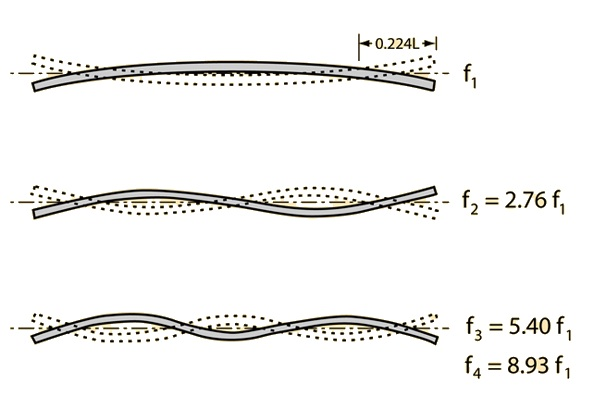
\includegraphics[width=.7\textwidth]{freebar.jpg}
\caption{
The first three transverse vibrational modes for 
a thin bar with free ends, and their corresponding
frequencies.
(Figure taken from 
{\tt hyperphysics.phy-astr.gsu.edu/}.)}
\label{f:freebar}
\end{center}
\end{figure}

\i The frequencies of the different transverse 
vibrational modes for a thin bar 
(length $L$, thickness $t$) with free ends are given by
%
\be
f_n = 0.1134\, m^2\,\frac{vt}{L^2}\,,
\quad{\rm where}\quad
m = 3.011,\ 5,\ 7,\ \cdots,\ (2n+1),\ \cdots
\ee
%
and $v=\sqrt{E/\rho}$ is the wave velocity in the bar.
($E$ is called {\em Young's modulus} and $\rho$ is 
the mass density (mass/volume) of the bar, both of 
which depend on the material.
$E$ is basically a spring constant for a 
bar under tension, defined by $F/A = E \Delta l/l$
for small displacements $\Delta l$.)

\i In terms of the fundamental frequency $f_1$, the 
frequencies of the partials are given by
%
\be
f_1\,,
\quad
f_2=2.76\,f_1\,,
\quad
f_3=5.40\,f_1\,,
\quad
f_4= 8.93\,f_1\,,
\quad
\cdots
\quad
f_n = \left(\frac{2n+1}{3.011}\right)^2\,f_1\,,
\quad
\cdots
\ee
%
Note that these frequencies are {\em not} harmonically
related to the fundamental frequency.
 
\i One can also set up {\em longitudinal} 
vibrations in a bar or rod, whose modes have a
simple harmominc relation:
%
\be
f_n = n\frac{v}{2L}\,,
\quad
{\rm where}\quad
n=1,\ 2,\ \cdots
\ee
%
This formula is identical in form to that for
standing waves on a stretched string, with 
$v=\sqrt{\tau/\mu}$ replaced by $v=\sqrt{E/\rho}$.

\i \demo Strike a 440~Hz thin bar supported over
a resonator box.
Where do you think the supports are located?

\i \demo Set up longitudinal vibrations in a long
thin rod by holding the middle of the rod between
your thumb and forefinger, while stroking the rod
with your other hand.
(You might need to wear a rosin-covered glove to
get enough friction to excite the longitudinal 
vibrations.)

\ei
%%%%%%%%%%%%%%%%%%%%%%%%%%%%%%%%%%%%%%%%%
\subsection{Glockenspeil, xylophone, marimba, vibraphone}
\bi

\i Glockenspiel bars are rectangular.
Since the bars are supported at the nodes of the 
fundamental vibration mode, the fundamental frequency 
is the dominant pitch for a glockenspiel bar.

\i Xylophone, marimba and vibraphone bars are 
``scooped out" near the center of the bar, 
forming an arch.
In this narrower section of the bar, the sound 
waves travel slower, decreasing the frequency of 
the transverse vibrational modes.

\i The arch serves two purposes:
(i) since the vibrational frequencies are lower,
one can get the lower pitches without needing
excessively long bars;
(ii) the arch allows one to tune the overtone
frequencies to harmonics of the fundamental.

\i For xylophones, the first overtone is tuned
to the 3rd harmonic of the fundamental.
For marimbas and vibraphones, the arch is 
deeper and tunes the first overtone to the 
4th harmonic.

\i The xylophone, marimba, and vibraphone also
have {\em resonator tubes} below each bar, whose 
lengths are chosen to match the fundamental 
frequencies of the different bars.

\i The resonator tubes increase the loudness
of the sound at the expense of a
shorter decay time for the vibrations of the bars.
(The tubes efficiently couple the vibration of the
bars to motion of the surrounding air.)

\i Since the natural frequencies of the 
resonator tubes are harmonics of the fundamental
frequency of the tube, the resonator tubes select out 
the fundamental and any {\em harmonically-related} 
frequencies associated with the vibrations of the bars.
 
\i The resonator tubes of a vibraphone have
motor-driven discs that alternately open and
close, producing a vibrato effect associated 
with the changing intensity of the sound.
The speed of the motor can be adjusted in order
to produce a slow vibrato or fast vibrato.
A vibraphone is sometimes played without vibrato
by turning the motor off.

\ei
%%%%%%%%%%%%%%%%%%%%%%%%%%%%%%%%%%%%%%%%%%%%%%%
\subsection{Chimes and triangles}
\bi

\i Chimes are long vertical pipes (rods) 
that are typically struck near the top.

\i The perceived {\em strike tone} for a 
chime is the missing
fundamental for modes $n=4,\ 5,\ 6$.
These modes have relative frequencies 
$9^2:11^2:13^2$, which are approximately 
equal to $2:3:4$.

\i A triangle is a thin solid metal rod that 
is bent in the shape of a triangle.  
When struck, the tone produced is similar to 
that of a straight rod of the same length.

\ei
%%%%%%%%%%%%%%%%%%%%%%%
\subsection{Vibrating membranes}
\bi

\i A vibrating membrane is the 2-dimensional
analogue of a (1-dimensional) vibrating string.

\i Since a membrane is a 2-dimensional object,
the modes of oscillation are labeled by two 
integers $(m,n)$.
For circular membranes,
$m=0,1,2,\cdots$ specifies the number of nodal diameters and 
$n=0,1,2,\cdots$ specifies the number of nodal 
circles.
(If the membrane is fixed at the circumference, 
$n$ starts at 1.)

\i Figures~\ref{f:membrane} and \ref{f:membrane2} 
show several vibrational modes of an
ideal circular membrane, fixed at the circumference
like a drumhead.
Adjacent parts of the membrane move in opposite
directions.
%
\begin{figure}[htbp]
\begin{center}
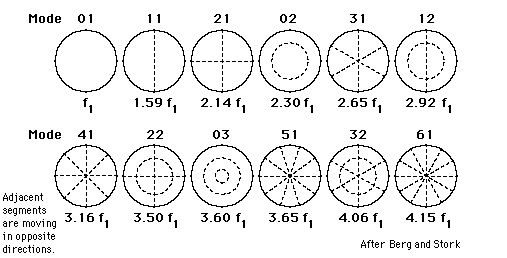
\includegraphics[width=.9\textwidth]{membrane.jpg}
\caption{
Several vibrational modes of an 
ideal circular membrane, fixed at the circumference.
The modes are labelled by two integers $(m,n)$,
where $m$ is the number of nodal diameters and
$n$ is the number of nodal circles.
Also given are the vibrational frequencies of
each mode in terms of the fundamental frequency $f_1$.
(Figure taken from 
{\tt http://www.mwit.ac.th/~physicslab/}, adapted
from ``Physics of sound," by Berg and Stork.)}
\label{f:membrane}
\end{center}
\end{figure}
%
\begin{figure}[htbp]
\begin{center}
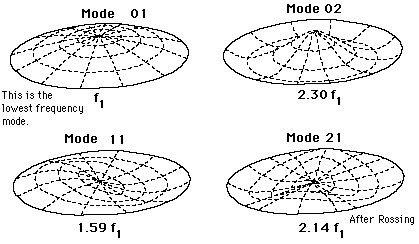
\includegraphics[width=.7\textwidth]{membrane2.jpg}
\caption{A perspective view of the first 
four vibrational modes of an ideal circular
membrane, fixed at the circumference.
See also Figure~\ref{f:membrane}.
(Figure taken from 
{\tt http://www.mwit.ac.th/~physicslab/}.)}
\label{f:membrane2}
\end{center}
\end{figure}

\i The frequencies of the different vibrational
modes for an ideal circular membrane of radius $r$
fixed at the circumference are given by
%
\be
f_{mn} = \frac{v}{2\pi r}\,x_{mn}\,,
\quad m=0, 1, 2, \cdots
\quad n=1, 2, 3, \cdots
\ee
%
where $v=\sqrt{\tau/\sigma}$ is the wave velocity
on the membrane.
($\tau$ is the tension and $\sigma$ is the 2-dimensional
mass density (mass/area) of the membrane.)

\i Technical note:
$x_{mn}$ denotes the $n$th zero of a special 
function called a {\em Bessel function} $J_m(x)$,
which is similar to a damped sinusoid.
The values of $x_{mn}$ determine the relative
frequencies of the vibrational modes, some of
which are given in Figures~\ref{f:membrane}
and \ref{f:membrane2}.

\i In terms of the fundamental frequency $f_1$, the
frequencies of the first few partials are given by
%
\be
f_{01} = f_1\,,\quad 
f_{11} = 1.59f_1\,,\quad 
f_{21} = 2.14f_1\,,\quad
f_{02} = 2.30f_1\,,\quad
f_{31} = 2.65f_1\,,\quad
\cdots
\ee
%
Note that these frequencies are {\em not} harmonically
related, just as we saw for the transverse vibrational
modes of a thin bar or rod.

\i \demo 
{\tt http://en.wikipedia.org/wiki/Vibrations\_of\_a\_circular\_membrane}
has an animation of the various vibrational modes of a circular membrane: 

\i Drums are the prime example of percussion instruments 
that use vibrating membranes as their source of sound.

\i The membrane is usually made out of animal skin or
some type of synthetic material, like mylar.

\ei
%%%%%%%%%%%%%%%%%%%%%%%%%%%%%%%%%%%%%%%%\
\subsection{Timpani}
\bi

\i Timpani (or kettle drums) consist of a circular membrane
stretched across the top of kettle-shaped enclosure.
There are tension screws along the circumference of the 
drum head and a foot pedal, both of which can be used to 
change the tension in the drum head.

\i A timpani drum head does not behave like an ideal 
membrane due to: (i) some inherent stiffness associated with the 
material of the membrane, and (ii) its interaction with the air 
enclosed in the kettle.
The inherent stiffness tends to raise the frequency 
of the higher vibrational modes, while the interaction with the air
tends to lower the frequency of the lower vibrational modes.

\i These two features tend to bring the overtones into 
a near harmonic relationship.
The frequencies of the dominant modes 
(1,1), (2,1), (3,1), (4,1) for a real kettle drum
have the approximate ratio
$1:1.5:2:2.5$ or, equivalently, $2:3:4:5$, which is
part of a harmonic series.
(The (0,1) mode is not relevant, since it dies down 
quickly because it motion tries to change the total 
air volume in the kettle.)

\i These (nearly harmonic) modes give the timpani its 
strong sense of pitch.

\i NOTE: Some people perceive the missing 
fundamental ($0.5 f_{11}$) as the pitch associated with 
these modes.
Others perceive the pitch to equal just $f_{11}$.
It depends on the strength of the partials 
$f_{21}$, $f_{31}$, and $f_{41}$ relative to $f_{11}$.

\ei
%%%%%%%%%%%%%%%%%%%%%%%
\subsection{Bass drum, tomtom, snare drum}
\bi

\i A bass drum is a large two-headed drum.

\i The tension in the two heads (the {\em batter head},
which is struck, and the {\em carry head}, on the 
other side) is adjusted differently in 
order to produce an indefinite pitch.

\i The vibrations of the two drum heads are coupled 
by the enclosed air.

\i Tomtoms are either single-headed or two-headed
drums of various sizes.
Like the bass drum, tomtoms have an indefinite pitch.

\i A snare drum is basically a tomtom with 
{\em snares} (wires) stretched across the drum head
opposite the batter head (called the {\em snare head}).

\i The vibrations of the batter head are coupled 
to the snare head and the snares via the enclosed air 
between the two drum heads.

\ei
%%%%%%%%%%%%%%%%%%%%%%%
\subsection{Vibrating plates}
\bi

\i A vibrating plate is similar to a vibrating membrane, 
with the restoring force coming from the inherent 
stiffness of the plate and not from an external tension.

\i Figure~\ref{f:plate} shows several vibrational
modes of a 15-in cymbal, which is behaves like a
thin circular plate that is supported at the center 
and is free at the circumference.
The vibrational modes are labelled by integers
$(m,n)$, similar to that for circular membranes.
%
\begin{figure}[htbp]
\begin{center}
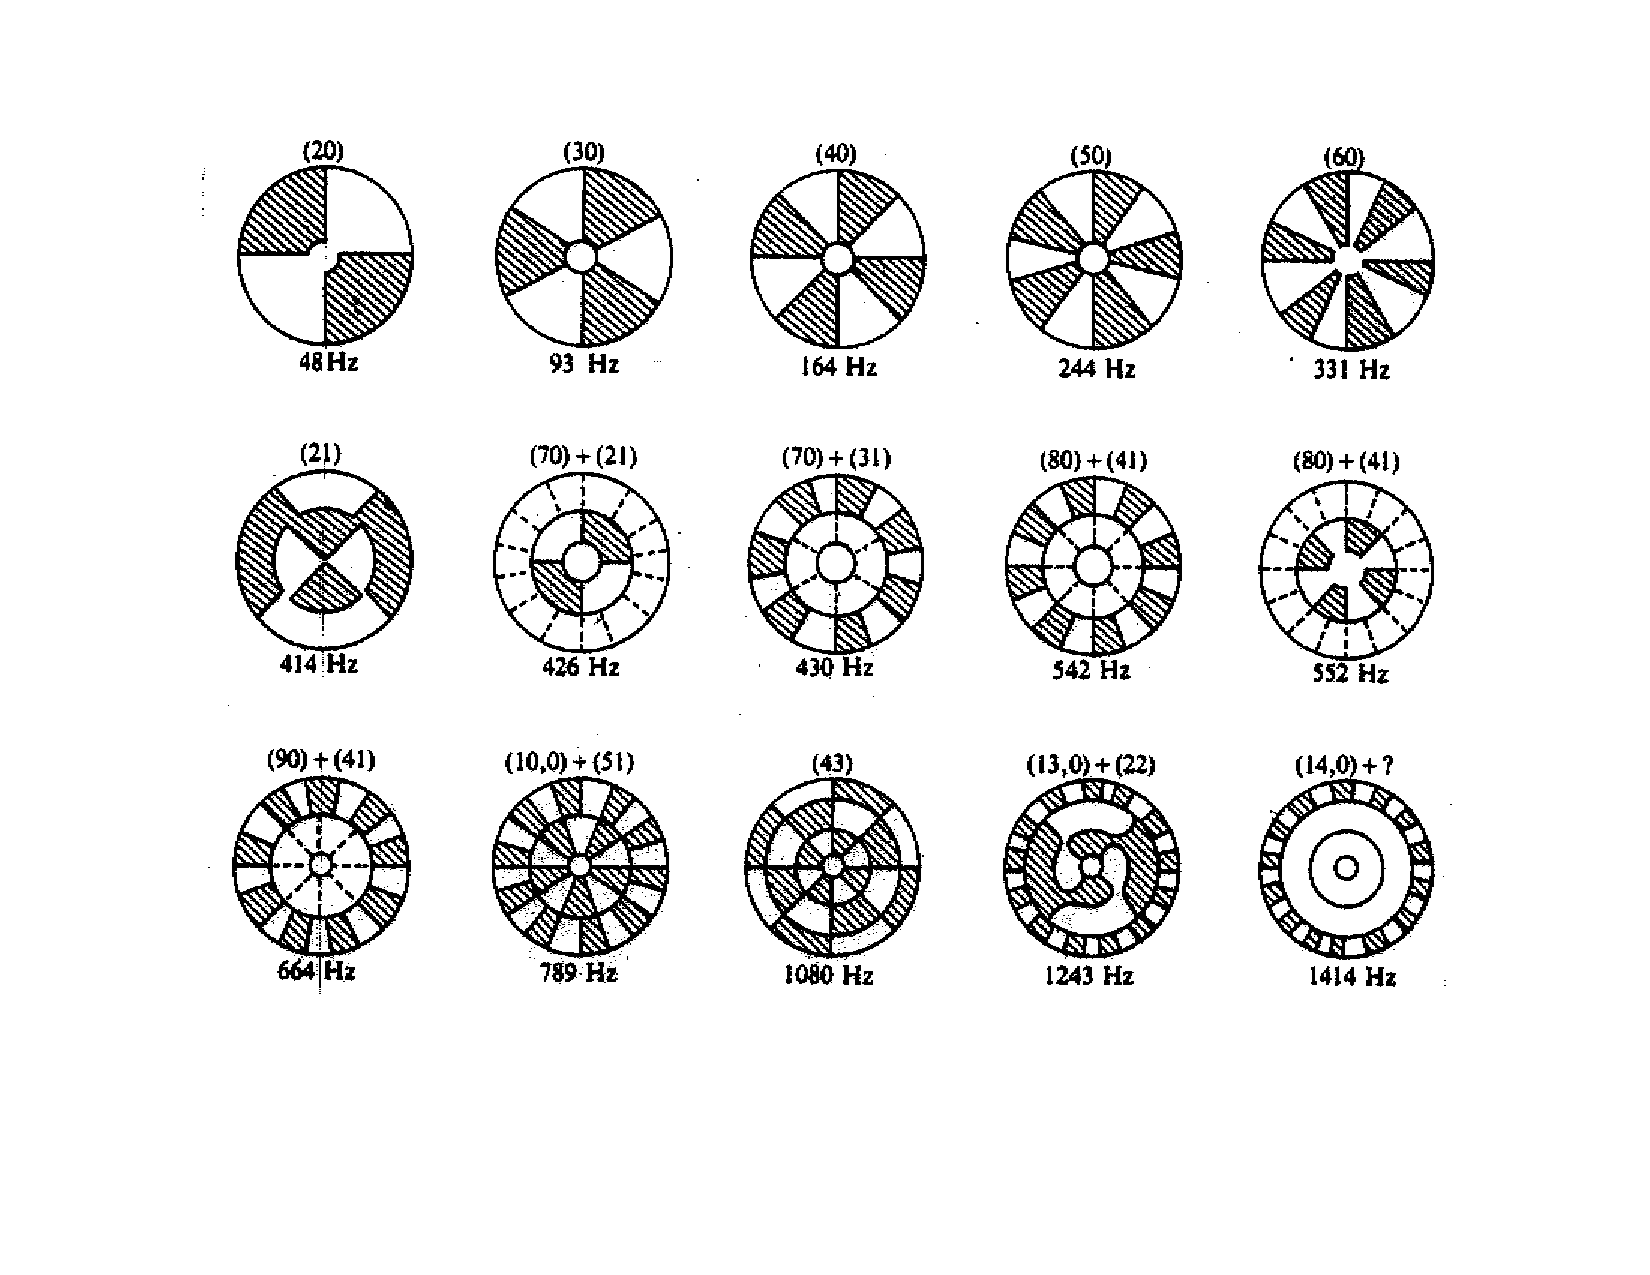
\includegraphics[width=.9\textwidth]{plate.pdf}
\caption{
Several vibrational modes of a 15-in 
cymbal that is supported at the center and is 
free at the circumference.
The first six vibrational patterns are for 
single modes;
the remaining patterns are for combinations of
two or more modes.
Also given are the frequencies of the various
vibrational modes.
(Figure taken from ``Science of Sound," by
Rossing, Moore, and Wheeler.)}
\label{f:plate}
\end{center}
\end{figure}
%

\i Cymbals, gongs, and bells are all examples of
vibrating plates.

\i E.F.F.~Chladni (in 1827) noticed that one can
illustrate various vibrational modes of a thin 
plate by bowing the edge of the plate, 
supported at the center, with fine sand (or salt) 
sprinkled on top of the plate.
As the plate vibrates, the sand accumulates along 
the nodal lines of the vibrational mode.

\i \demo The YouTube video 
{\tt http://www.youtube.com/watch?v=wMIvAsZvBiw}
shows various vibrational patterns for a thin
square metal plate.
These vibrational patterns are sometimes called 
{\em Chladni patterns} after E.F.F.~Chladni.

\i \demo
Repeat the YouTube video demonstration in class for 
both a square plate and circular plate.

\ei
%%%%%%%%%%%%%%%%%%%%%%%%%
\subsection{Cymbals and gongs}
\bi

\i A cymbal is a thin disc of metal with a slight 
bulge in the center where it is supported.

\i The high-energy crash of two cymbals excites many
high and low frequency vibrational modes.
The sound that is produced has an indefinite pitch.

\i After crashing two cymbals together, the musician
holds the cymbals with their faces pointing outward
toward the audience.  
This is because the direction of the radiated sound 
is predominantly {\em perpendicular}
to the face of the cymbals, in the direction of the
vibrations of the metal disc.

\i Gongs are flat discs of metal with the edges 
turned over to form a ridge (sort of like a metal 
trash can cover).
They produce sound with a fairly definite pitch.

\i Non-linear effects in both cymbals and gongs transfer 
energy from one vibrational mode to another, making the 
pitch change with time (usually from low to high).

\ei
%%%%%%%%%%%%%%%%%%%%%%%%%%%%%%%%%%%%%%%%%%%%%%
\subsection{Bells}
\bi

\i Bells are circular plates whose edges have 
been bent so that several of the overtones are in near
harmonic relation with one another.

\i Figure~\ref{f:bell} show several vibrational
modes of a large church bell.
The lower circles show the vibrational modes at the
rim of the bell.
The marks show the location of nodal points on the rim.
%
\begin{figure}[htbp]
\begin{center}
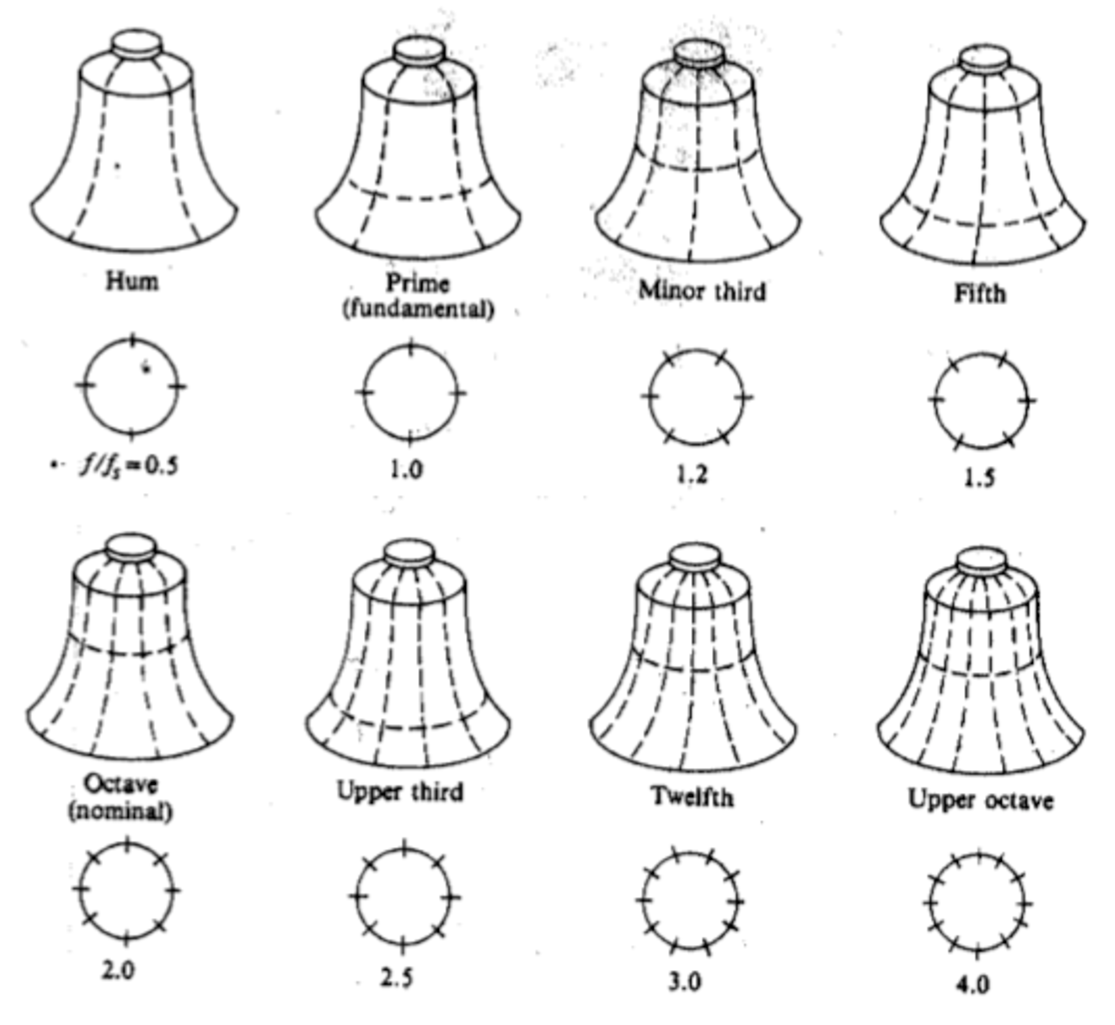
\includegraphics[width=.8\textwidth]{bell.pdf}
\caption{
Several vibrational modes of a large church bell.
The lower circles show the vibrational modes at the
rim of the bell.
Also given are the frequencies of the various
vibrational modes in terms of the prime (fundamental) mode.
(Figure taken from ``Science of Sound," by
Rossing, Moore, and Wheeler.)}
\label{f:bell}
\end{center}
\end{figure}
%

\i Similar to chimes, the strike note of a bell is the 
missing fundamental for the harmonically-related 
octave, twelfth, and upper octave overtones having
frequency ratios $2:3:4$.
Although there is an actual vibration mode (called the
{\em prime} mode) whose 
frequency coincides with the missing fundamental, 
the perceived pitch is predominantly due to the other
frequencies.

\ei

